\documentclass{scrartcl}


\usepackage{texenv}
\begin{document}

%title
%\noindent\makebox[\linewidth]{\rule{\textwidth}{0.2pt}}
{\Large \centering \textsf{IT-Systeme: "Ubungsblatt 06} -- Florian Macherey, 
\today}\\
\noindent\makebox[\linewidth]{\rule{\textwidth}{0.2pt}} \\

%\normalsize \flushleft

\section*{Aufgabe 1: Rechnerarchitekturen}
\subsection*{1a) Was ist der Unterschied zwischen einem ccNUMA- und 
einem SMP Rechner?}
Die Abk"urzung ccNUMA steht f"ur \textit{cache coherent non-uniform 
Memory 
Access}. Es bedeutet das Prozessoren von Mulitprozessorsystemen jeweils 
einen 
eigenen Adressraum haben, aber anderen Prozessoren Zugriff darauf 
gew"ahren. 
Cache Koh"arenz hei\ss t hierbei, wenn ein Prozessor Daten aus einem 
anderen 
Cache lie\ss t und ver"andert, m"ussen die ge"anderten Daten danach mit 
den 
anderen Caches synchronisiert werden. \\
Nicht koh"arente Systeme sind zwar 
einfacher zu realisieren, sind aber nicht effizient als Von-Neumann-Rechner 
zu 
bauen. 

\section*{Aufgabe 2: Randomisierte Algorithmen}
{\large{Gegeben sei folgernder Graph, dessen Koordinaten im 
$X-Y-$Koordinatensystem 
liegen: $(1,5); (4,7); (2,7); (3,1)$}} \\
\textit{Annahme: Die Kosten zwischen den Konten werden als die 
euklisische 
Norm zwischen zwei Knoten 
angenommen.} \\
Damit ergeben sie folgende Kosten:
\begin{align*}
A \leftrightarrow B\colon& ~||B-A||_2 = \sqrt{3^2 + 2^2} &&= \sqrt{13} 
\approx 
3.605551275\\
A \leftrightarrow C\colon& ~||C-A||_2 = \sqrt{1^2 + 4^2} &&= \sqrt{5} 
\approx 
2.23.6067977 \\
A \leftrightarrow D\colon& ~||D-A||_2 = \sqrt{2^2 + (-4)^2} &&= 
\sqrt{20} 
\approx 
4.472135955 \\
B \leftrightarrow C\colon& ~||C-B||_2 = \sqrt{(-2)^2 + 0^2} &&= \sqrt{4} 
= 2 \\
B \leftrightarrow D\colon& ~||D-B||_2 = \sqrt{(-1)^2 + (-6)^2} &&= 
\sqrt{37} 
\approx 6.08276253 \\
C \leftrightarrow D\colon& ~||D-C||_2 = \sqrt{1^2 + (-6)^2} &&= 
\sqrt{37} 
\approx 
6.08276253
\end{align*}
\begin{center}
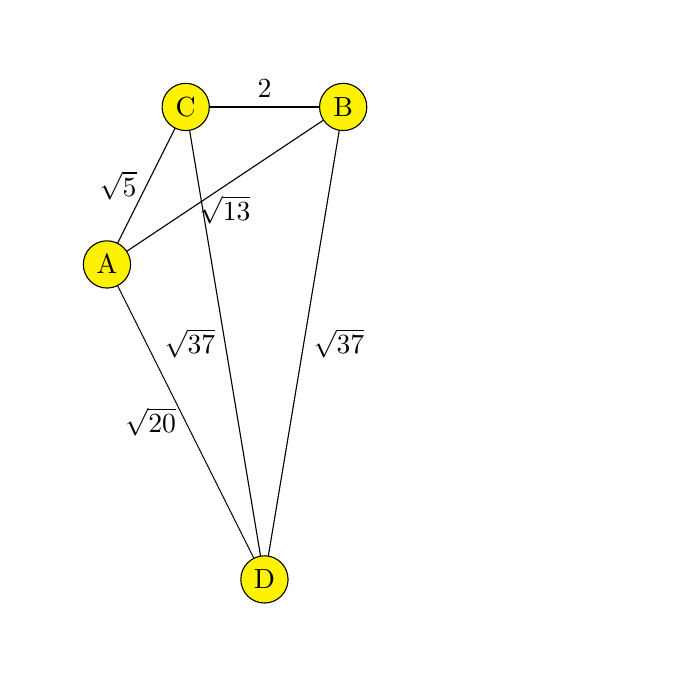
\begin{tikzpicture}
\coordinate[](A) at (1,5);
\coordinate[](B) at (4,7);
\coordinate[](C) at (2,7);
\coordinate[](D) at (3,1);
\draw[white] (0,0) rectangle (8,8);

\path[draw] (A)--(B) node[midway, anchor=north] {$\sqrt{13}$};
\path[draw] (A)--(C) node[midway, anchor=east] {$\sqrt{5}$};
\path[draw] (A)--(D) node[midway, anchor=east] {$\sqrt{20}$};
\path[draw] (B)--(C) node[midway, anchor=south] {$2$};
\path[draw] (B)--(D) node[midway, anchor=west] {$\sqrt{37}$};
\path[draw] (C)--(D) node[midway, anchor=east] {$\sqrt{37}$};

\draw[fill=yellow] (A) circle (0.3) node {A};
\draw[fill=yellow] (B) circle (0.3) node {B};
\draw[fill=yellow] (C) circle (0.3) node {C};
\draw[fill=yellow] (D) circle (0.3) node {D};
\end{tikzpicture}
\end{center}

\subsection*{2a) Finden sie per Hand die k"ureste Rundreise des 
Problems.}
Wenn man die k"urzeste Rundreise per Hand bestimmt, ist diese $D 
\rightarrow A 
\rightarrow C \rightarrow B \rightarrow D$, mit den Kosten: $K_{shortest} 
\approx 
14.79086646\ldots$. 

\subsection*{2b) Verwenden Sie die 
\textit{Nearest-Neighborhood-Heuristik}, um eine Rundreise zu bestimmen}
Mit dieser Heurisik ergibt sich f"ur den Knoten $A$ als Startknoten die 
Rundreise 
$A \rightarrow C \rightarrow B \rightarrow D \rightarrow A$ mit den Kosten 
$K_{NNH} \approx 14.79086646\ldots$ damit ist $K_{NNH} = 
K_{shortest}$. 

\subsection*{2c) Vergleichen sie ihre Ergebnisse aus a) und b) hinsichtlich 
ihrer G"ute}
Die erste Variante findet immer den k"urzesten Weg, hat also die beste 
m"ogliche 
G"ute. Die \textit{Nearest-Neighborhood-Heuristik} liefert in der Regel eine 
schlechte L"osung, da immer der n"achste, noch nicht besuchte Knoten 
besucht 
wird. Dabei kann es vorkommen, dass dann zwischen dem letzten und dem 
Startknoten die Kosten sehr gro\ss ~sind. Die optiomale Strategie w"are 
\textit{All-Nearest-Neighbors}, wobei von jedem Knoten die g"unstigeste 
Rundreise gesucht wird. Dieser h"atte aber eine zu aufwendgie Laufzeit. \\
Da in diesem Graphen alle Punkte miteinander verbunden sind und im 
$\mathbb{R}^2$ liegen bzw. in Beziehung stehen, ist die k"urzeste 
Rundreise die konvexe H"ulle der vier Punkte. Somit findet die 
\textit{Nearest-Neighborhood-Heuristik} hier 
auch die bestm"ogliche L"osung.

\section*{Aufgabe 3: Zufall}
\subsection*{3a) Er"ortern Sie, warum es auf einem handels"ublichen 
Computer keinen \dq echten\dq ~Zufall gibt.}
Es gibt auf handels"ubichen Computern keine echten Zufallszahlen, da 
diese Zahlen algorithmisch erzeugt werden. Sie liefern f"ur den gleichen 
Startwert auch 
immer 
die gleiche Zahlenfolge. Deswegen werden die meisten 
Zufallszahlengeneratoren 
auch Pseudozufallszahlengeneratoren genannt. 

\subsection*{3b) Was bedeutet dies f"ur einen randomisierten 
Algorithmus?}
Da es keinen echten Zufall gibt, m"ussen diese Algorithmen entweder auf 
\texttt{/dev/random}\footnote{Unter Linux ist random blockierend, unter 
FreeBSD nicht, unter Mac OS sind random und urandom "aquivalent 
(http://en.wikipedia.org/?title=/dev/random)} zur"uckgreifen oder einen 
unabh"angigen Startwert 
nehmen. 
Daf"ur eignet sich zum Beispiel der UNIX-Timestamp. Wenn die 
Algorithmen nicht 
mit echten Zufallszahlen als Startwerte benutzt werden, k"onnen diese nicht 
ihre 
Effizienz durch zuf"allig richtige Ergbnisse ausnutzen.

\subsection*{3c) Welche Hilfmittel k"onnen verwendet werden, um den \dq 
echten\dq ~Zufall auf einem Computer zu realisieren.}
Wie schon unter 3b) geschrieben, kann der echte Zufalls durch 
kryptographische 
Zufallszahlen verbessert werden. Daf"ur wird in der Regel das 
\texttt{/dev/random} genutzt. Diese Zufallszahlen werden unter anderm 
aus den 
Ger"auschen von Ger"atetreibern oder Mausbewegungen erzeugt. Sie sind 
damit 
echte Zufallszahlen.

\section*{Aufgabe 4: Quantencomputer}
{\large{Erkl"aren Sie folgende Begriffe:
\begin{enumerate}
\item Superposition
\item Quantenverschr"ankung
\end{enumerate}}}
Unter Superposition versteht man, dass sich die Amplituden der 
Quantenteilchen 
"uberlagern. Normalerweise k"onnen diese nur 0 oder 1 sein, wenn sie aber 
gleichzeitig und "uberlagernd sind, entsteht diese Superposition. Die 
Quantenverschr"ankung bedeutet, dass Teilchen nicht mehr unabh"angig 
voneinander betrachtet werden k"onnen, sondern dass sich "Anderungen 
auf 
ein 
Teilchen auch auf die anderen verschr"ankten Teilchen auswirken. 

\section*{Aufgabe 5: Monte-Carlo Algorithmus - Beispielanwendung}
{\large{Schreiben Sie ein Programm(Java oder C), welches die Kreiszahl $\pi$ 
n"ahrungsweise mit Hilfe von Zufallszahlen bestimmt.}}
\lstinputlisting[language=C,otherkeywords={clock\_t,time\_spent},]{ue06.05/main.c}
Ausgabe:
\begin{lstlisting}
Iterationen        100 Werte: Pi: 3.141593, berechneter Wert: 3.200000, 
Differenz: 5.840735e-02, Laufzeit: 0.00000600
Iterationen       1000 Werte: Pi: 3.141593, berechneter Wert: 3.136000, 
Differenz: 5.592654e-03, Laufzeit: 0.00002800
Iterationen      10000 Werte: Pi: 3.141593, berechneter Wert: 3.172800, 
Differenz: 3.120735e-02, Laufzeit: 0.00027200
Iterationen     100000 Werte: Pi: 3.141593, berechneter Wert: 3.144880, 
Differenz: 3.287346e-03, Laufzeit: 0.00275100
Iterationen    1000000 Werte: Pi: 3.141593, berechneter Wert: 3.144212, 
Differenz: 2.619346e-03, Laufzeit: 0.02524200
Iterationen   10000000 Werte: Pi: 3.141593, berechneter Wert: 3.141438, 
Differenz: 1.542536e-04, Laufzeit: 0.24798100
Iterationen  100000000 Werte: Pi: 3.141593, berechneter Wert: 3.141495, 
Differenz: 9.813359e-05, Laufzeit: 2.43916800
Iterationen 1000000000 Werte: Pi: 3.141593, berechneter Wert: 3.141616, 
Differenz: 2.342241e-05, Laufzeit: 24.39983000
\end{lstlisting}



\end{document}
